%% Example document for the eis_msc_thesis document class. Compile with
%% pdfLaTeX or LaTeX.
%%
%% Created: April 7, 2004, by Johan Carlson
%% Last modified: June 7, 2009, by Johan Carlson


%% Pick one of the following depending on the language of the report, and if 
%% you want twosided or onesided print.
%% Also change language definition after \begin{document}

% English, twosided
\documentclass[12pt,a4paper,openright,final,twoside,en]{csee_msc_thesis} 

% English, onesided    
%\documentclass[12pt,a4paper,openright,final,oneside,en]{csee_msc_thesis}     

% Swedish, twosided
%\documentclass[12pt,a4paper,openright,final,twoside,sv]{csee_msc_thesis}     

% Swedish, onesided
%\documentclass[12pt,a4paper,openright,final,oneside,sv]{csee_msc_thesis}     

%%==================================================================
%% Class options specific to this class
%%==================================================================
%%   en, sv  - Swedish or English
%%   parskip - Use blank row instead of indentation for
%%             new paragraphs
%%==================================================================

%% These packages are not required in general,
%% only for some examples in this document.
\usepackage{fancybox}
\usepackage{verbatim}

\begin{document}

%%==================================================================
%% Define variables here
%%==================================================================

\def\thesistitle{An Example Master's Thesis}
\def\theauthor{Johan E.\ Carlson}
\def\theaddress{Lule� University of Technology\\
            Dept.\ of Computer Science and Electrical Engineering\\
            Div.\ of Systems and Interaction}

% Define the English abstract
\def\theabstract{ProMoVis provides an environment where engineers may, through a combination of graphical visualisation and powerful analysis tools, analyse and deepen their understanding of complex processes and its components. Currently a drawback is that the user has to create a model of the system, through the graphical interface that ProMoVis provides, even though he may have existing models created in another environment.\\\newline This report describes the design process and implementation of a tool, written in python, that utilizes the JModelica environment to export models, described in Modelica, to an equivalent SFG representation used in ProMoVis. This is done through linearising a model around an operating point and then extracting a DAE representation of it. From this DAE, it is then possible to extract an SFG representation, describing how a component depends on other components in the system.\\\newline Besides demonstrating the key algorithm for extracting the SFGs this report also discusses the design of the software and how the internals of the tool is divided into separate phases. Phases responsible for compiling the original model, building an intermediate representation of the SFGs for internal use, validation of the system together with some optional transformations of the original model and finally the actual generation of the ProMoVis representation from the intermediate representation. }
\def\thepreface{I worked on this project during the spring of 2012 starting out as a novice in the field of control theory and physical modeling with only the most fundamental knowledge in the subject. But having been in touch with Modelica in earlier courses, and found it to be a powerful tool that I would like to deepen my understanding of. It was not hard to accept when Wolfgang Birk proposed this project.\\\newline The source code to the tool is currently available at https://github.com/jwmbrg/Modelica-to-PromoVis-export, although I probably will move the actual export software to a separate repository, without the school related information, for continued development after this project has ended.\\\newline I would like to thank Wolfgang Birk and Miguel Casta{\~{n}}o for the time and effort they have put down,  with their pragmatic approach, they have been invaluable in giving me a deepened understanding of the field of control theory and mathematical modeling.\\\newline Finally, I would like to give credit to Johan Carlson for providing the \LaTeX{} template used in formatting this report. \\\newline Hopefully the output of the project, the export tool, might help make ProMoVis more accessible to existing users of Modelica and also provide a foundation for a tighter integration between the two environments.\\\newline
\vspace*{2cm}%
\hfill Jesper Moberg
}
\def\thedate{Template version: \theclassversion , \theclassdate}

% Use this if you want a Swedish abstract
%\def\theswedishabstract{\input{SweAbstract/sweabstract.tex}}

%%==================================================================
%% Generate preamble pages here (This should not need any changes)
%%==================================================================
\startpreamble
  {\thesistitle}
  {\theauthor}
  {\theaddress}
  {\theabstract}
  {\thepreface}
  {\thedate}
 % {\theswedishabstract} % use this for Swedish abstract, leave empty for English

%%==================================================================
%% Start including the chapters
%%==================================================================
% First argument is the "running titles", second is the chapter name.
\makechapter{Introduction}{Introduction\label{ch1}}
\section{Background}
%During a research project at LTU a tool was developed, called ProMoVis,  aimed at structure analysis and visualisation of complex physical processes.
While Modelica, Simulink and other existing tools are very powerful when it comes to simulation and modelling of  dynamic systems there is a need for a tool that can aid engineers in selecting different control structures by making it possible to analyse specific interconnections in dynamic systems. %A drawback with existing tools is that although a user declares the relations between inputs and outputs, at simulation time the models are still assumed to be treated as "black boxes". Making it hard to monitor and analyse the internal behaviour of components in the modelled systems. 
Due to the identified need for a tool that can solve these problems \cite{ProMoVisPaper}\nocite{*}, the design and implementation of ProMoVis started in 2010 which recently was released as an open source project.
\section{Problem Description}
As stated earlier, ProMoVis purpose is visualisation and analysis of large systems. It assumes that the user has information about the components of the system and the relations between them.  Today, %there is no scripting interface to ProMoVis and 
models have to be created in the graphical environment by placing the components and defining the relations one by one. This is a task that can become very tedious and error-prone for many systems. At the same time a user that would benefit from using ProMoVis in his design process can be assumed to already have existing models, from another environment, available. Therefore the possibility to import existing models would make ProMoVis more accessible to its intended users.
\section{Project Goal}
In recent time Modelica, as a tool for modeling of physical systems, has shown an increase in popularity and has become somewhat of a standard for describing physical systems. Due to its widespread use and the amount of open source tools that are available for models described with help from the language, this projects goal is to implement a tool that can import models, described in Modelica, into ProMoVis. This tool should try to preserve as much information and semantics from the original Modelica models but, at the same time, keep the effort needed from the user to perform the export at a minimum. A final demand is that the tool should be easy to integrate with the existing ProMoVis environment so that imports can be performed from within ProMoVis.
% Features needed
%There is a need to a tool for control structure selection. It should analyse the interconnections in a dynamic system and how a control strategy should be shaped. This very different from what you write here.]





\makechapter{The second chapter}{The second chapter\label{ch2}}
\section{Workflow}
During the projects initial phase much of the time was put on familiarizing with the ProMoVis and JModelica enviroments and the math that acts as a foundation for the Modelica models. During these first weeks there were sporadic meetings and discussions with the supervisor whenever problems or questions appeared. After an initial meeting with the developer of the ProMoVis frontend (See Appendix \ref{appC}). The start of the development of a first "Proof of concept" was initiated. After finishing this, a more thorough design phase started where both the developers of ProMoVis and a "test-user" got involved in the process. 
\section{Tools}
\subsection{Modelica}
Modelica is a object-oriented declarative programming language used to create models of physical system. Unlike many other modelling languages, Modelica is not domain specific and thus can be used to model physical systems consisting of a mix of electrical, mechanical and chemical processes. Since the release of the first language specification in 1997 the continuous development of the language has been maintained by the Modelica Association and the current version of the Language specification is 3.2 \cite{ModelicaSpec}.\nocite{*}
\subsection{JModelica}
There is several environments, both proprietary and open source, that provides tools for compilation, analysis and simulation of  models described in Modelica. Since the use of proprietary software would demand that we separate the export tool from ProMoVis. An initial demand on the environment to be used was that it should be open source. After examining the options available JModelica\cite{jmodelicaorg}\nocite{*} was choosen because of its Python front-end, that makes it easy to interface with the tool from other software while still providing a structured environment around which we can build all parts of the export tool.   
\subsection{Numpy and SciPy}
Another important feature supporting the use of the JModelica platform was its tight integration with the NumPy and SciPy packages \cite{scipyorg}\nocite{*}. These are two very popular open source packages for Python providing a strong and well documented toolbox for mathematical computing. When extracting the mathematical models through JModelica they are represented using the data-structures provided by NumPy and in many cases this removes the need to "reinvent the wheel" for many of the operations that needs to be performed on the mathematical models before export. Instead one can directly use existing methods provided by SciPy and NumPy. The use of this package also makes the source-code for the export tool more accesible to other programmers familiar with Python and these packages.
\subsection{The SFG}
Since the SFG is a fundamental concept in ProMoVis it is motivated to give a brief introduction to how it is used in ProMoVis. ProMoVis bases its analysis and visualisation on SFG representations of dynamical systems. It is this representation the tool needs to be able to accurately extract from the existing Modelica models. Basically the an SFG is a directed graph with the vertices representing each of the states in the systems and the edges representing the relation, in terms of transfer functions, between the vertices.\\\newline The simple two tank system in Fig.~\ref{fig:twotank} Can be described by the general equations.

\begin{figure}

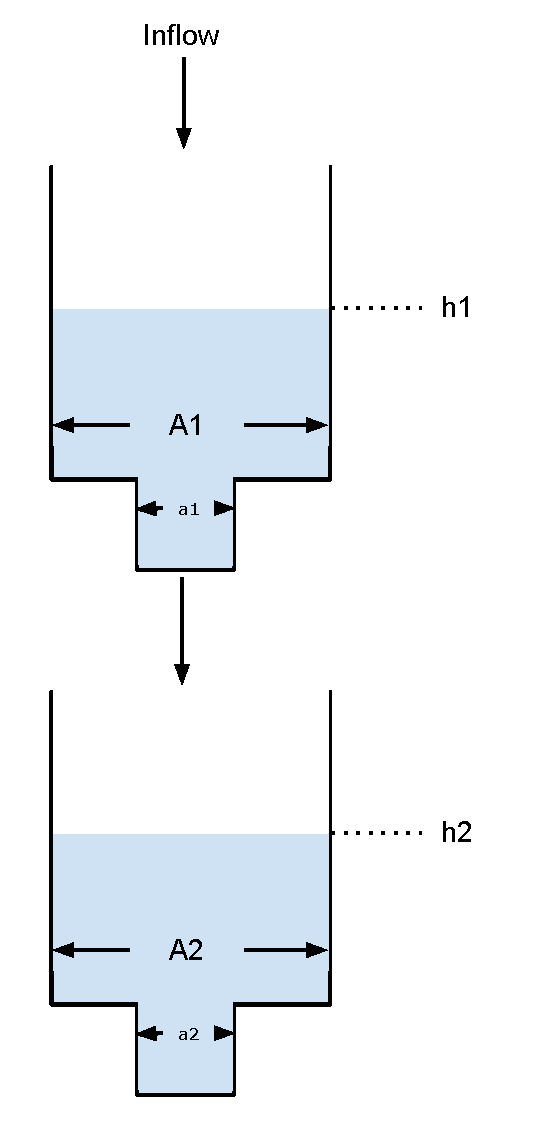
\includegraphics[scale=0.4,bb=0 0 3.67in 7.47in] {Figures/TwoTankSystem.pdf}\\\newline
\caption{A simple two tank system}
\label{fig:twotank}
\end{figure}
\begin{equation}
    \dot{h_1} = -a_1/A_1*\sqrt{2*g*h_1} + inflow\\\newline
\end{equation}
\begin{equation}
	\dot{h_2} = -a_2/A_2*\sqrt{2*g*h_2} + a_1/A_1*\sqrt{2*g*h_1}
\end{equation}
Linearising the specific model, described in Modelica,  in Appendix \ref{appD}. We can then extract the transfer functions. For the parameters specified the following is obtained:\\\newline
Transfer function from inflow to h1 is : $\begin{array}{rcl} \frac{1}{s +2.3*10^{-2}} \end{array}$\\\newline
Transfer function from h1 to h2 is :$\begin{array}{rcl} \frac{2.3*10^{-2}}{s +8.9*10^{-2}} \end{array}$\\\newline
And the corresponding signal flow graph, as shown in Fig.~\ref{fig:sfg}, can be obtained. From the figure, it is easy to see that the vertices in the SFG is the states of the system and the edges are the transfer functions between the states. In ProMoVis, there is also additional information supplied with the vertices, such as operating point, saturation values etc. 
\begin{figure}
\fbox{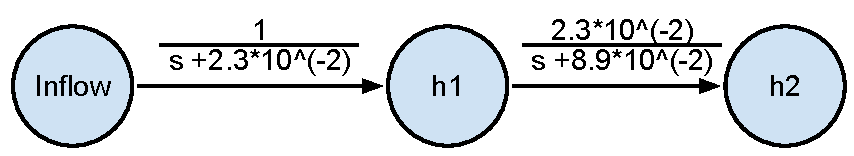
\includegraphics[scale=0.8,bb=0 0 5.69in 1.04in] {Figures/sfgtwotank.pdf}}
\caption{Corresponding SFG for the two tank system in Fig~\ref{fig:twotank}}
\label{fig:sfg}
\end{figure}


%%==================================================================
%% Include any appendices here.
%%==================================================================
\appendix % This command initializes the appendix part, Don't change!

%% Include appendix A, add more if needed
\makeappendix{Appendix A}{Least squares fit of response surface
models by multiple linear regression\label{appA}}

\section{Deciding which variable to solve first}
When extracting the SFGs from the DAE one has to make sure that one solves each of the rows for the correct variables making sure that you can extract an SFG for every variable in the system.Recall the general equation for the DAE:
\begin{equation}
E*dx = A*x + B*u + F*w + g
\end{equation}
If no algebraic equations are present in the orignal Modelica model, the resulting DAE would have the following form:
\begin{equation}
E*dx = A*x + B*u + g
\end{equation}
The number of rows in such a system, containing no algebraic variables, would be the same as the amount of the number of declared or inferred states in the systems. The introduction of algebraic variables, that we recall are all variables that does not have a declared derivative, adds 1 row to the DAE.Since states, by definition, has a derivative declared, we can therefore look only at the E and F matrices to solve the problem of which row to solve for which variable. Since a state has to be solved for a row containing its derivative. If we declare:
\begin{equation}
S=[E|F]
\end{equation}
Here we easilly realize that the S matrix will be an nxn matrix, since we by concatenating the E and F matrix, add as many columns that there is extra rows.\\
With the column vector L
\begin{equation}
L=[dx_0...dx_i, w_0...w_i]
\end{equation}
We then examine this system:
\begin{equation}
S*L
\end{equation}
By examining each of the columns in S and storing all the rownumbers that contains non-zero elements together with the variable corresponding to the column a list is retrieved for each of the variables.This  list i containing all the rownumbers where the variable is present.
The pseudocode for this process might look something like this:
\begin{lstlisting}
varDict.initWithKeysAndValues(L,[])
for row in S {
	for col in row{
		if(col.value !=0){
			key=L(numberOf(col));
			value=numberOf(row)
			list=varDict(key)
			list.append(value)		
		}
	}			
}
\end{lstlisting}
As one can see, this approach has a quadratic running time, no matter the input, compared to a pure gaussian elimination approach, that has a cubic time complexity.

The task is then to start extracting the SFGs from the original DAE with the help of this list. If the system contains no algebraic loops, it should be possible to iterate through the dictionary and find a variable that has only one rownumber associated with it. Removing that variable from the dictionary and remove the corresponding rownumber from the remaining variables in the dictionary.

Pseudocode for this process:
\begin{lstlisting}
int i=0
int looped=0 // looped is used to detect algebraic loops
solvList=[]
while(varDict!=empty && looped !=2) {
	key=varDict(i).key
	list=varDict(key)
	if(lengthOf(list)==1){
		//add a tuple with rownumber and key
		rowNumber=list[0]
		solvList.append((key,rowNumber);
		//remove the key (variable), since the
		// problem is solved for this key
		varDict.remove(key)
		
		for otherLists in varDict{
			//we remove the rownumber 
			//from the rest of the variables.
			//Since this row is already consumed
			//in the solution
			otherLists.remove(rowNumber)
		}
		looped=0; 	//If we solved for a variable, 
					//reset looped.
	}
	i=i+1;
	if(i>varDict.size()){
		i=0; //restart the process from the beginning
		looped+=1; // increment looped 	
	}			
}
if(looped==2){
	print "failed due to algebraic loops
}else{
	print "success"
}

\end{lstlisting}

At this point, we have a list of tuples, with each of the tuples containing a variable name and a row number, and we can begin to extract the SFGs from the DAE by solving each of the variable for the given rownumber.

%%==================================================================
%% Include bibliography references here
%% Replace the "thesisreferences" with your
%% own reference database
%%==================================================================
\bibliographystyle{ieeetr}

\fancyhead[LO]{}%
\fancyhead[RE]{}%
\fancyhead[LE]{\thepage}%
\fancyhead[RO]{\thepage}
\bibliography{thesisreferences}

\end{document}
